77. \begin{figure}[ht!]
\center{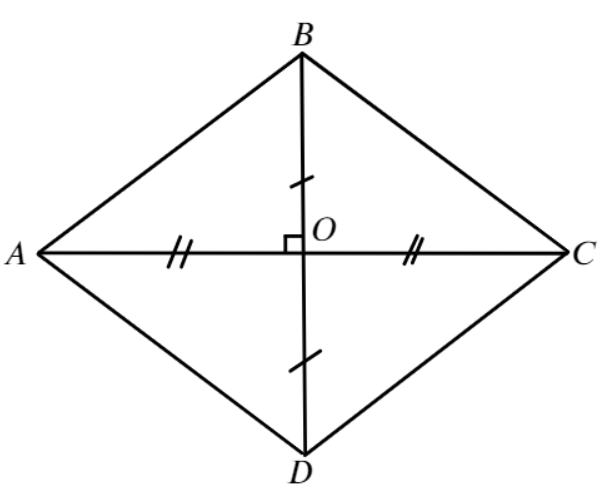
\includegraphics[scale=0.35]{g8-76.png}}
\end{figure}\\
В ромбе диагонали перпендикулярны и делятся (как и в любом параллелограмме) точкой пересечения пополам. Пусть $AC=18,$ тогда $AO=16:2=8$ и по теореме Пифагора $BO=\sqrt{AB^2-AO^2}=\sqrt{100-64}=6,$ значит $BD=2BO=12.$\\
